\documentclass[aspectratio=169,11pt,t]{beamer}

% ============================================================
% Theme and typography
% ============================================================

\usetheme{Madrid}
\usecolortheme{default}
\usefonttheme{professionalfonts}

\setbeamertemplate{navigation symbols}{}
\setbeamertemplate{headline}{}

\setbeamertemplate{footline}{%
  \leavevmode\hbox{%
  \begin{beamercolorbox}[wd=.82\paperwidth,ht=2.5ex,dp=1.0ex,leftskip=.8em]{author in head/foot}
    CSCI 6461 --- Computer Systems Architecture
  \end{beamercolorbox}%
  \begin{beamercolorbox}[wd=.18\paperwidth,ht=2.5ex,dp=1.0ex,rightskip=.8em]{date in head/foot}
    \hfill\insertframenumber/\inserttotalframenumber
  \end{beamercolorbox}}
}

\setbeamersize{
  text margin left=0.65cm,
  text margin right=0.65cm
}

\setbeamerfont{frametitle}{size=\Large, series=\bfseries}
\setbeamerfont{block title}{size=\normalsize, series=\bfseries}
\setbeamertemplate{blocks}[rounded][shadow=false]

% Block vertical padding adjustments
\addtobeamertemplate{block begin}{\vspace{0.1em}}{\vspace{0.1em}}
\addtobeamertemplate{block end}{}{\vspace{0.2em}}

% Base list item separation
\setbeamertemplate{itemize/enumerate body begin}{\setlength{\itemsep}{4pt}}
\setbeamertemplate{itemize/enumerate subbody begin}{\setlength{\itemsep}{2pt}}

% ============================================================
% Packages
% ============================================================

\usepackage[T1]{fontenc}
\usepackage{lmodern}
\IfFileExists{sourcecodepro.sty}{\usepackage[scale=0.92]{sourcecodepro}}{\usepackage{courier}}
\usepackage{amsmath}
\usepackage{booktabs}
\usepackage{array}
\usepackage{colortbl}
\usepackage{tikz}

\usetikzlibrary{
  arrows.meta,
  positioning,
  shapes.geometric,
  calc,
  decorations.pathreplacing
}

% ============================================================
% Colors
% ============================================================

\definecolor{navy}{RGB}{24,43,68}
\definecolor{deepblue}{RGB}{45,88,130}
\definecolor{lightblue}{RGB}{235,242,250}
\definecolor{softgray}{RGB}{245,247,250}
\definecolor{darkgray}{RGB}{25,28,32}
\definecolor{gold}{RGB}{200,145,35}

\setbeamercolor{palette primary}{bg=navy,fg=white}
\setbeamercolor{palette secondary}{bg=deepblue,fg=white}
\setbeamercolor{frametitle}{bg=navy,fg=white}
\setbeamercolor{title}{fg=white}
\setbeamercolor{subtitle}{fg=white}
\setbeamercolor{author}{fg=white}
\setbeamercolor{date}{fg=white}
\setbeamercolor{titlelike}{fg=white}
\setbeamercolor{block title}{bg=deepblue,fg=white}
\setbeamercolor{block body}{bg=lightblue,fg=darkgray}
\setbeamercolor{normal text}{fg=darkgray,bg=white}

% ============================================================
% Formatting shortcuts
% ============================================================

\setlength{\parskip}{0pt}

\newcommand{\key}[1]{\textbf{#1}}
\newcommand{\bits}[1]{\texttt{#1}}
\newcommand{\hex}[1]{\texttt{0x#1}}
\newcommand{\code}[1]{\texttt{#1}}
% Simple fixed-width bit-field box for instruction diagrams.
% Coordinates use bit positions; set x scale in the tikzpicture.
\newcommand{\bfld}[5]{%
  \pgfmathsetmacro{\cx}{#1 + #3/2}%
  \fill[#5] (#1,#2) rectangle ++(#3,0.72);%
  \draw[navy,line width=0.7pt] (#1,#2) rectangle ++(#3,0.72);%
  \node[font=\scriptsize,align=center,text=darkgray] at (\cx,#2+0.36) {#4};%
}
\newcommand{\bitnote}[3]{%
  \node[font=\tiny,align=center,text=darkgray] at (#1,#2) {#3};%
}
\newcommand{\codeblock}[1]{%
  \begingroup\small\ttfamily\setlength{\fboxsep}{5pt}\colorbox{softgray}{\begin{minipage}{0.92\linewidth}#1\end{minipage}}\endgroup%
}


% Section divider macro
\newcommand{\sectiondivider}[2]{%
\begin{frame}[plain]

\begin{tikzpicture}[remember picture,overlay]
\fill[navy] (current page.south west) rectangle (current page.north east);
\fill[gold] (current page.south west)
  rectangle ([yshift=.15cm]current page.south east);
\end{tikzpicture}

\vspace*{\fill}

\begin{minipage}{0.94\textwidth}
\raggedright
\hyphenpenalty=10000
\exhyphenpenalty=10000

{\color{gold}\large\bfseries #1\par}

\vspace{0.3cm}

{\color{white}\fontsize{22}{26}\selectfont\bfseries
#2\par}

\end{minipage}

\vspace*{\fill}

\end{frame}
}

% ============================================================
% Metadata
% ============================================================

\title[Topic 7]{
  Machine Code \& AArch64 Instruction Encoding
}

\subtitle{
  Fixed-width instruction words, encoding fields, data-processing,\\
  memory access, and branch instructions
}

\author{
  Computer Systems Architecture
}

\date{}

% ============================================================
% Document
% ============================================================


\begin{document}

% ============================================================
% Slide 1
% ============================================================

\begin{frame}[plain]

\begin{tikzpicture}[remember picture,overlay]
\fill[navy] (current page.south west) rectangle (current page.north east);
\fill[gold] (current page.south west)
  rectangle ([yshift=.15cm]current page.south east);
\end{tikzpicture}

\vspace*{\fill}

\begin{minipage}{0.88\textwidth}

{\color{gold}\normalsize\bfseries
CSCI 6461 \;|\; Computer Systems Architecture \;|\; TOPIC 7
\par}

\vspace{0.25cm}

{\color{white}\fontsize{24}{28}\selectfont\bfseries
Machine Code \& AArch64\\[0.08cm]Instruction Encoding
\par}

\vspace{0.35cm}

{\color{white!80}\large
Instruction words, encoding fields, immediates, memory operations,\\and branch targets in AArch64
\par}

\end{minipage}

\vfill

{\color{white!70}\small
Dr. J. Burns
\par}

\vspace*{\fill}

\end{frame}

% ============================================================
% Slide 2
% ============================================================

\begin{frame}{Topic 7 Outline}

\setbeamertemplate{enumerate item}{\arabic{enumi}.}

\begin{enumerate}\setlength{\itemsep}{8pt}
  \item \key{Machine Code and 32-bit Instruction Words}
  \begin{itemize}
    \item Assembly text, instruction words, bit fields, and byte order.
  \end{itemize}
  \item \key{AArch64 Encoding Families}
  \begin{itemize}
    \item How high-order bits select data-processing, load/store, and branch formats.
  \end{itemize}
  \item \key{Data-Processing Encodings}
  \begin{itemize}
    \item Register operands, immediate operands, and worked examples.
  \end{itemize}
  \item \key{Memory and Branch Encodings}
  \begin{itemize}
    \item Load/store offsets, PC-relative addressing, unconditional branches, and conditional branches.
  \end{itemize}
\end{enumerate}

\end{frame}

% ============================================================
% Slide 3
% ============================================================

\sectiondivider{Topic 7}{Machine Code and 32-bit Instruction Words}

% ============================================================
% Slide 4
% ============================================================

\begin{frame}{From Assembly to Machine Code}

\begin{itemize}\setlength{\itemsep}{6pt}
  \item A processor repeatedly \key{fetches}, \key{decodes}, and \key{executes} instructions.
  \item During fetch--decode--execute, the processor fetches a 32-bit instruction word from memory and interprets its bit fields.
  \item This topic starts with the earlier step: how an AArch64 assembly instruction is encoded as that fixed \key{32-bit} machine instruction.
\end{itemize}

\vspace{0.18cm}

\begin{center}
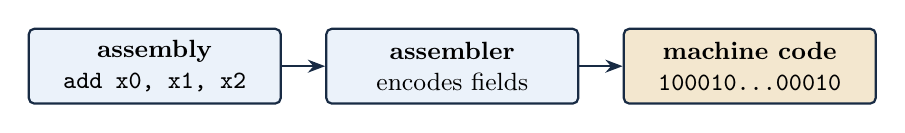
\begin{tikzpicture}[
  font=\small,
  node distance=0.55cm,
  procbox/.style={
    draw=navy,
    line width=0.8pt,
    rounded corners=2pt,
    minimum width=3.2cm,
    minimum height=0.95cm,
    align=center,
    fill=lightblue
  },
  wordboxstyle/.style={
    procbox,
    fill=gold!22
  },
  arr/.style={
    -{Stealth[length=2.2mm]},
    draw=navy,
    line width=0.8pt
  }
]

\node[procbox] (asm) {\textbf{assembly}\\\code{add x0, x1, x2}};
\node[procbox, right=of asm] (assembler) {\textbf{assembler}\\encodes fields};
\node[wordboxstyle, right=of assembler] (wordbox) {\textbf{machine code}\\\bits{100010\ldots00010}};

\draw[arr] (asm) -- (assembler);
\draw[arr] (assembler) -- (wordbox);

\end{tikzpicture}
\end{center}

\end{frame}

% ============================================================
% Slide 5
% ============================================================

\begin{frame}{AArch64 vs. AArch32 Encoding}

\begin{columns}[T,onlytextwidth]

\column{0.48\textwidth}
\begin{block}{Shared 32-bit Structure}
\begin{itemize}\setlength{\itemsep}{5pt}
  \item Instructions are encoded as fields inside a 32-bit word.
  \item Different instruction classes use different field layouts.
  \item A small number of high-level formats helps the decoder.
\end{itemize}
\end{block}

\column{0.48\textwidth}
\begin{block}{AArch64 Encoding}
\begin{itemize}\setlength{\itemsep}{5pt}
  \item There is no 4-bit condition field in every instruction.
  \item Register fields are usually 5 bits because there are 32 integer registers.
  \item The high-order bits identify a broader encoding family.
\end{itemize}
\end{block}

\end{columns}

\vspace{0.25cm}

\vspace{0.1cm}

Machine code is a structured 32-bit word whose fields the processor decodes.

\end{frame}

% ============================================================
% Slide 6
% ============================================================

\begin{frame}{AArch64 Instruction Word Basics}

\vspace{-0.15cm}

Each AArch64 instruction is 32 bits, or 4 bytes. Four consecutive
instructions therefore occupy two 64-bit memory rows.

\vspace{0.2cm}

\begin{center}
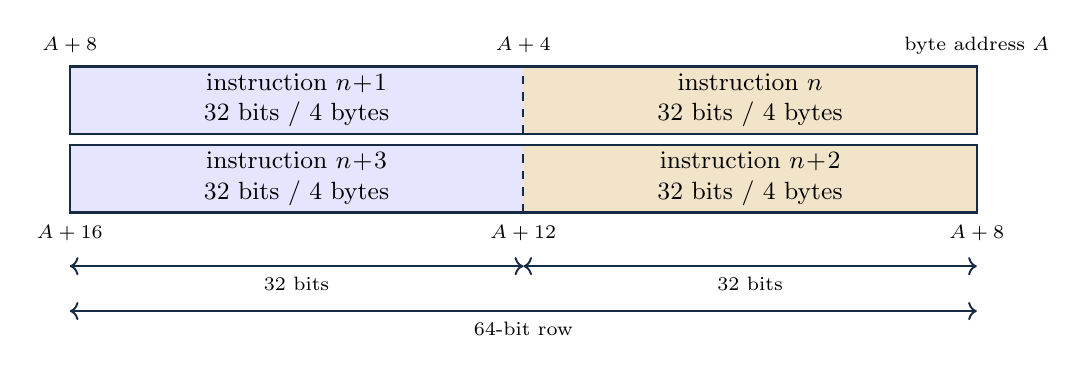
\begin{tikzpicture}[x=0.18cm,y=0.95cm]

  % top row
  \fill[blue!10] (0,1.05) rectangle (32,1.95);
  \fill[gold!25] (32,1.05) rectangle (64,1.95);
  \draw[navy, line width=0.9pt] (0,1.05) rectangle (64,1.95);
  \draw[navy, dashed, line width=0.8pt] (32,1.05) -- (32,1.95);

  % bottom row
  \fill[blue!10] (0,0) rectangle (32,0.9);
  \fill[gold!25] (32,0) rectangle (64,0.9);
  \draw[navy, line width=0.9pt] (0,0) rectangle (64,0.9);
  \draw[navy, dashed, line width=0.8pt] (32,0) -- (32,0.9);

  \node[align=center, font=\small] at (48,1.50)
    {instruction $n$\\32 bits / 4 bytes};
  \node[align=center, font=\small] at (16,1.50)
    {instruction $n\!+\!1$\\32 bits / 4 bytes};
  \node[align=center, font=\small] at (48,0.45)
    {instruction $n\!+\!2$\\32 bits / 4 bytes};
  \node[align=center, font=\small] at (16,0.45)
    {instruction $n\!+\!3$\\32 bits / 4 bytes};

  % addresses, shown with low-order bits/lowest byte address on the right
  \node[font=\scriptsize] at (64,2.23) {byte address $A$};
  \node[font=\scriptsize] at (32,2.23) {$A+4$};
  \node[font=\scriptsize] at (0,2.23) {$A+8$};
  \node[font=\scriptsize] at (64,-0.28) {$A+8$};
  \node[font=\scriptsize] at (32,-0.28) {$A+12$};
  \node[font=\scriptsize] at (0,-0.28) {$A+16$};

  % width labels
  \draw[navy, <->, line width=0.7pt] (0,-0.72) -- (32,-0.72);
  \node[font=\scriptsize] at (16,-0.95) {32 bits};
  \draw[navy, <->, line width=0.7pt] (32,-0.72) -- (64,-0.72);
  \node[font=\scriptsize] at (48,-0.95) {32 bits};
  \draw[navy, <->, line width=0.7pt] (0,-1.32) -- (64,-1.32);
  \node[font=\scriptsize] at (32,-1.56) {64-bit row};

\end{tikzpicture}
\end{center}

\vspace{-0.15cm}

\begin{block}{Instruction Boundaries}
Each instruction starts 4 bytes after the previous one. A 64-bit memory row
holds two AArch64 instructions.
\end{block}

\end{frame}

% ============================================================
% Slide 7
% ============================================================

\begin{frame}{How the Decoder Starts}

\begin{itemize}\setlength{\itemsep}{6pt}
  \item AArch64 has several major encoding families.
  \item The decoder first checks high-order opcode bits to select the family.
  \item After the family is known, the remaining fields can be interpreted.
\end{itemize}

\vspace{0.15cm}

\textbf{Examples of instruction families}

\vspace{0.05cm}

\begin{itemize}\setlength{\itemsep}{4pt}
  \item Data processing: arithmetic, logical, moves, shifts, and compares.
  \item Load/store: memory access through base registers and offsets.
  \item Branch: unconditional branches, calls, returns, and conditional branches.
\end{itemize}

\vspace{0.1cm}

Identify the broad instruction family first, then read the fields that belong to
that family.

\end{frame}

% ============================================================
% Slide 8
% ============================================================

\sectiondivider{Topic 7}{Common Encoding Fields and Conditional Patterns}

% ============================================================
% Slide 9
% ============================================================

\begin{frame}{Common AArch64 Encoding Prefixes}

\small
AArch64 has no single universal opcode field. Fixed high-order bits identify
the instruction form, and the remaining bits encode operands.

\vspace{0.1cm}

\begin{center}
\scriptsize
\rowcolors{2}{lightblue!70}{white}
\begin{tabular}{@{}lll@{}}
\toprule
Instruction form & Fixed high-order bits & Remaining fields \\
\midrule
\code{add x, x, x}     & \bits{10001011000} & \code{Rm}, shift, \code{Rn}, \code{Rd} \\
\code{sub x, x, x}     & \bits{11001011000} & \code{Rm}, shift, \code{Rn}, \code{Rd} \\
\code{add x, x, \#imm} & \bits{10010001}    & shift, \code{imm12}, \code{Rn}, \code{Rd} \\
\code{sub x, x, \#imm} & \bits{11010001}    & shift, \code{imm12}, \code{Rn}, \code{Rd} \\
\code{ldr x, [x, \#imm]} & \bits{1111100101} & \code{imm12}, \code{Rn}, \code{Rt} \\
\code{str x, [x, \#imm]} & \bits{1111100100} & \code{imm12}, \code{Rn}, \code{Rt} \\
\code{b label}         & \bits{000101}       & \code{imm26} \\
\code{bl label}        & \bits{100101}       & \code{imm26} \\
\code{b.cond label}    & \bits{01010100}     & \code{imm19}, \code{cond} \\
\bottomrule
\end{tabular}
\end{center}

\vspace{0.08cm}

\textbf{Reading the table:} these prefixes identify the form; they are not complete instructions. Operand fields fill the remaining bits.

\end{frame}

% ============================================================
% Slide 10
% ============================================================

\begin{frame}{Conditional Execution in AArch64}

\small
\begin{itemize}\setlength{\itemsep}{4pt}
  \item AArch32 allowed a condition code on most instructions; AArch64 does not.
  \item AArch64 uses conditional branches and selected conditional operations instead.
  \item Conditions are evaluated from the NZCV flags set by earlier arithmetic or compare instructions.
\end{itemize}

\vspace{0.12cm}

\begin{block}{Example}
\centering
\code{cmp x0, x1}
\quad$\longrightarrow$\quad
\code{b.lt less}
\quad\text{or}\quad
\code{csel x2, x3, x4, eq}
\end{block}

\vspace{0.1cm}

\begin{center}
\scriptsize
\rowcolors{2}{blue!6}{white}
\begin{tabular}{@{}ll@{\hspace{0.75cm}}ll@{}}
\toprule
Condition & Meaning & Condition & Meaning \\
\midrule
\code{eq} / \code{ne} & equal / not equal
  & \code{ge} / \code{lt} & signed $\ge$ / $<$ \\
\code{hs} / \code{lo} & unsigned $\ge$ / $<$
  & \code{gt} / \code{le} & signed $>$ / $\le$ \\
\code{hi} / \code{ls} & unsigned $>$ / $\le$
  & \code{mi} / \code{pl} & negative / non-negative \\
\bottomrule
\end{tabular}
\end{center}

\vspace{0.12cm}

Conditional behavior remains, but the 4-bit condition field is no longer attached to most instructions.

\end{frame}

% ============================================================
% Slide 11
% ============================================================

\begin{frame}{From AArch32 Predication to AArch64 Conditions}

\small

AArch32 ARM instructions usually reserved bits 31:28 for a condition field.
That made most instructions conditionally executable.

\vspace{0.2cm}

\begin{center}
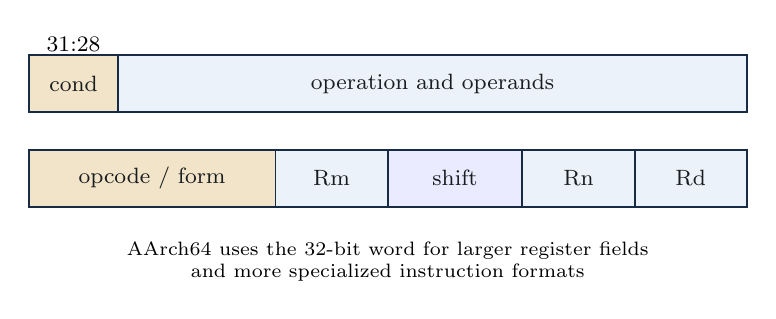
\begin{tikzpicture}[x=0.285cm,y=1cm]

  % AArch32 layout
  \bfld{0}{0.95}{4}{\footnotesize cond}{gold!25}
  \bfld{4}{0.95}{28}{\footnotesize operation and operands}{lightblue}

  \node[font=\footnotesize, anchor=south] at (2,1.6) {31:28};

  % AArch64 layout
  \bfld{0}{-0.25}{11}{\footnotesize opcode / form}{gold!25}
  \bfld{11}{-0.25}{5}{\footnotesize Rm}{lightblue}
  \bfld{16}{-0.25}{6}{\footnotesize shift}{blue!8}
  \bfld{22}{-0.25}{5}{\footnotesize Rn}{lightblue}
  \bfld{27}{-0.25}{5}{\footnotesize Rd}{lightblue}

  \node[font=\scriptsize, align=center] at (16,-0.95)
    {AArch64 uses the 32-bit word for larger register fields\\and more specialized instruction formats};

\end{tikzpicture}
\end{center}

\vspace{0.12cm}

AArch64 no longer attaches a 4-bit condition field to most instructions.
Conditional behavior is handled with conditional branches and selected
conditional operations.

\end{frame}

% ============================================================
% Slide 12
% ============================================================

\begin{frame}{Conditional Examples in AArch64}

\small

AArch64 does not have a general \code{add.lt} form.

\vspace{0.18cm}

\noindent
\begin{minipage}[t]{0.48\textwidth}
\vspace{0pt}
\begin{block}{Move if less than}
\code{cmp x0, x1}\\[2pt]
\code{csel x2, x3, x2, lt}

\vspace{0.1cm}

If \code{x0 < x1}, then \code{x2} gets \code{x3}; otherwise \code{x2}
keeps its old value.
\end{block}
\end{minipage}
\hfill
\begin{minipage}[t]{0.48\textwidth}
\vspace{0pt}
\begin{block}{Add if less than}
\code{cmp x0, x1}\\[2pt]
\code{b.ge skip}\\[2pt]
\code{add x2, x2, \#1}\\[2pt]
\code{skip:}

\vspace{0.1cm}

The \code{add} executes only when \code{x0 < x1}.
\end{block}
\end{minipage}

\vspace{0.12cm}

Use conditional selection when choosing between values; use a branch when the
arithmetic instruction itself should be conditional.

\end{frame}

% ============================================================
% Slide 13
% ============================================================

\sectiondivider{Topic 7}{Data-Processing Instruction Encodings}

% ============================================================
% Slide 14
% ============================================================

\begin{frame}{Data Processing: Register Form}

\begin{block}{Example Instruction}
\[
\code{add x5, x6, x7}
\]
\end{block}

\vspace{0.1cm}

\begin{center}
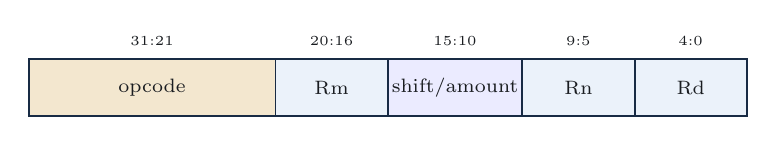
\begin{tikzpicture}[x=0.285cm,y=1cm]
  \bfld{0}{0}{11}{opcode}{gold!22}
  \bfld{11}{0}{5}{Rm}{lightblue}
  \bfld{16}{0}{6}{shift/amount}{blue!8}
  \bfld{22}{0}{5}{Rn}{lightblue}
  \bfld{27}{0}{5}{Rd}{lightblue}
  \bitnote{5.5}{0.95}{31:21}
  \bitnote{13.5}{0.95}{20:16}
  \bitnote{19}{0.95}{15:10}
  \bitnote{24.5}{0.95}{9:5}
  \bitnote{29.5}{0.95}{4:0}
\end{tikzpicture}
\end{center}

\vspace{0.15cm}

\begin{itemize}\setlength{\itemsep}{5pt}
  \item \code{Rd} is the destination register.
  \item \code{Rn} is the first source register.
  \item \code{Rm} is the second source register.
  \item Shift fields are available because this form supports shifted register operands.
\end{itemize}

\end{frame}

% ============================================================
% Slide 15
% ============================================================

\begin{frame}{Encoding Example: \texttt{add x5, x6, x7}}

\begin{columns}[T,onlytextwidth]

\column{0.48\textwidth}
\begin{block}{Register Numbers}
\[
\begin{aligned}
Rd &= x5 = 00101 \\
Rn &= x6 = 00110 \\
Rm &= x7 = 00111
\end{aligned}
\]
\end{block}

\column{0.48\textwidth}
\begin{block}{Operation Fields}
\[
\begin{aligned}
\text{operation} &= \text{add} \\
\text{operand size} &= 64\text{-bit} \\
\text{shift amount} &= 0
\end{aligned}
\]
\end{block}

\end{columns}

\vspace{0.2cm}

\begin{center}
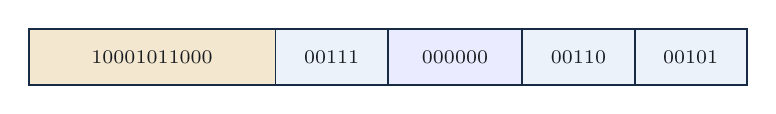
\begin{tikzpicture}[x=0.285cm,y=1cm]
  \bfld{0}{0}{11}{10001011000}{gold!22}
  \bfld{11}{0}{5}{00111}{lightblue}
  \bfld{16}{0}{6}{000000}{blue!8}
  \bfld{22}{0}{5}{00110}{lightblue}
  \bfld{27}{0}{5}{00101}{lightblue}
\end{tikzpicture}
\end{center}

\vspace{0.1cm}

\centering
The complete encoding is
\[
\bits{10001011000\;00111\;000000\;00110\;00101}
= \hex{8B0700C5}.
\]

\end{frame}

% ============================================================
% Slide 16
% ============================================================

\begin{frame}{Data Processing: Immediate Form}

\begin{block}{Example Instruction}
\[
\code{add x5, x6, \#24}
\]
\end{block}

\vspace{0.1cm}

\begin{center}
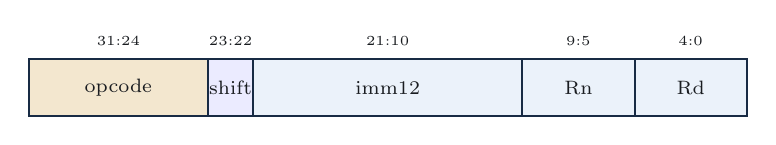
\begin{tikzpicture}[x=0.285cm,y=1cm]
  \bfld{0}{0}{8}{opcode}{gold!22}
  \bfld{8}{0}{2}{shift}{blue!8}
  \bfld{10}{0}{12}{imm12}{lightblue}
  \bfld{22}{0}{5}{Rn}{lightblue}
  \bfld{27}{0}{5}{Rd}{lightblue}
  \bitnote{4}{0.95}{31:24}
  \bitnote{9}{0.95}{23:22}
  \bitnote{16}{0.95}{21:10}
  \bitnote{24.5}{0.95}{9:5}
  \bitnote{29.5}{0.95}{4:0}
\end{tikzpicture}
\end{center}

\vspace{0.15cm}

\begin{itemize}\setlength{\itemsep}{5pt}
  \item The immediate field is 12 bits wide.
  \item The shift field can optionally shift the immediate by 12 bits.
  \item This format is common for address arithmetic and small integer constants.
\end{itemize}

\end{frame}

% ============================================================
% Slide 17
% ============================================================

\begin{frame}{Encoding Example: \texttt{add x5, x6, \#24}}

\begin{columns}[T,onlytextwidth]
\column{0.48\textwidth}
\begin{block}{Operands}
\[
\begin{aligned}
Rd &= x5 = 00101 \\
Rn &= x6 = 00110 \\
\text{imm12} &= 24 = 000000011000
\end{aligned}
\]
\end{block}

\column{0.48\textwidth}
\begin{block}{Instruction Meaning}
\[
\code{x5 = x6 + 24}
\]
The immediate value is part of the instruction word.
\end{block}
\end{columns}

\vspace{0.2cm}

\begin{center}
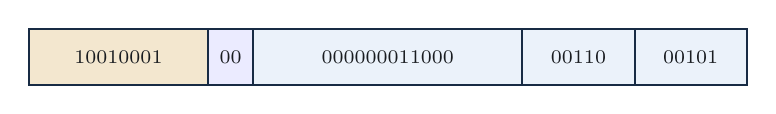
\begin{tikzpicture}[x=0.285cm,y=1cm]
  \bfld{0}{0}{8}{10010001}{gold!22}
  \bfld{8}{0}{2}{00}{blue!8}
  \bfld{10}{0}{12}{000000011000}{lightblue}
  \bfld{22}{0}{5}{00110}{lightblue}
  \bfld{27}{0}{5}{00101}{lightblue}
\end{tikzpicture}
\end{center}

\vspace{0.1cm}

\centering
\code{add x5, x6, \#24} is encoded as \hex{910060C5}.

\end{frame}

% ============================================================
% Slide 18
% ============================================================

\begin{frame}{AArch64 Immediate Encodings Are Specialized}

\begin{itemize}\setlength{\itemsep}{7pt}
  \item AArch64 does not use the AArch32 rotated-\code{imm8} data-processing scheme.
  \item Different instruction families have different immediate encodings.
  \item Some constants fit directly in an \code{add} or \code{sub} immediate.
  \item Other constants require move-wide instructions such as \code{movz}, \code{movn}, or \code{movk}.
  \item Logical instructions use their own bitmask-immediate encoding.
\end{itemize}

\vspace{0.2cm}

\begin{block}{Immediate Fields}
Do not ask whether a constant fits ``in AArch64'' in general. Ask whether it fits
in the specific immediate field of the instruction being used.
\end{block}

\end{frame}

% ============================================================
% Slide 19
% ============================================================

\sectiondivider{Topic 7}{Memory and PC-Relative Encodings}

% ============================================================
% Slide 20
% ============================================================

\begin{frame}{Load/Store Instruction Encoding}

\begin{block}{Example Instruction}
\[
\code{ldr x5, [x6, \#16]}
\]
\end{block}

\vspace{0.1cm}

\begin{center}
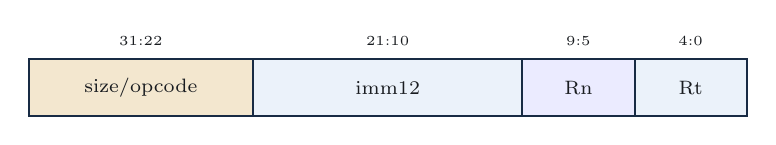
\begin{tikzpicture}[x=0.285cm,y=1cm]
  \bfld{0}{0}{10}{size/opcode}{gold!22}
  \bfld{10}{0}{12}{imm12}{lightblue}
  \bfld{22}{0}{5}{Rn}{blue!8}
  \bfld{27}{0}{5}{Rt}{lightblue}
  \bitnote{5}{0.95}{31:22}
  \bitnote{16}{0.95}{21:10}
  \bitnote{24.5}{0.95}{9:5}
  \bitnote{29.5}{0.95}{4:0}
\end{tikzpicture}
\end{center}

\vspace{0.1cm}

\begin{itemize}\setlength{\itemsep}{4pt}
  \item \code{Rt} is the register loaded or stored.
  \item \code{Rn} is the base address register.
  \item \code{imm12} is a scaled unsigned offset for this common form.
  \item For a 64-bit \code{ldr}: \(\text{address} = \code{x6} + 8 \times \text{imm12}\).
\end{itemize}

\end{frame}

% ============================================================
% Slide 21
% ============================================================

\begin{frame}{Encoding Example: \texttt{ldr x5, [x6, \#16]}}

\begin{columns}[T,onlytextwidth]
\column{0.48\textwidth}
\begin{block}{Operands}
\[
\begin{aligned}
Rt &= x5 = 00101 \\
Rn &= x6 = 00110 \\
\#16 &= 2 \times 8\text{ bytes}
\end{aligned}
\]
\end{block}

\column{0.48\textwidth}
\begin{block}{Encoded Offset}
\[
\text{imm12} = 2 = 000000000010
\]
The instruction stores the scaled value, not the byte offset directly.
\end{block}
\end{columns}

\vspace{0.2cm}

\begin{center}
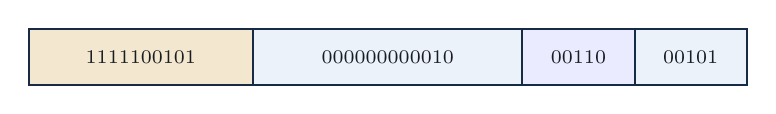
\begin{tikzpicture}[x=0.285cm,y=1cm]
  \bfld{0}{0}{10}{1111100101}{gold!22}
  \bfld{10}{0}{12}{000000000010}{lightblue}
  \bfld{22}{0}{5}{00110}{blue!8}
  \bfld{27}{0}{5}{00101}{lightblue}
\end{tikzpicture}
\end{center}

\vspace{0.1cm}

\centering
\code{ldr x5, [x6, \#16]} is encoded as \hex{F94008C5}.

\end{frame}

% ============================================================
% Slide 22
% ============================================================

\begin{frame}{Store Uses the Same Address Fields}

\small

\code{str x5, [x6, \#16]} is encoded as \hex{F90008C5}.

\vspace{0.2cm}

\begin{center}
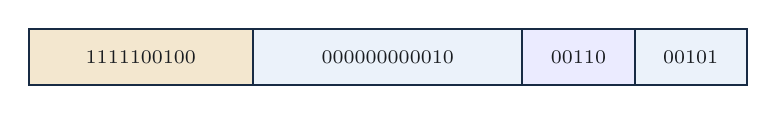
\begin{tikzpicture}[x=0.285cm,y=1cm]
  \bfld{0}{0}{10}{1111100100}{gold!22}
  \bfld{10}{0}{12}{000000000010}{lightblue}
  \bfld{22}{0}{5}{00110}{blue!8}
  \bfld{27}{0}{5}{00101}{lightblue}
\end{tikzpicture}
\end{center}

\vspace{0.15cm}

\begin{itemize}\setlength{\itemsep}{6pt}
  \item The base register and scaled offset fields match the load example.
  \item The operation field changes from load to store.
  \item \code{Rt} is now the source register whose value is written to memory.
\end{itemize}

\end{frame}

% ============================================================
% Slide 23
% ============================================================

\begin{frame}{Scaled Offsets Depend on Access Size}

\begin{block}{Unsigned Offset Form}
\[
\text{address} = \text{base} + \text{imm12} \times \text{access size}
\]
\end{block}

\vspace{0.15cm}

\begin{center}
\small
\begin{tabular}{lll}
\toprule
Instruction kind & Access size & Encoded immediate meaning \\
\midrule
\code{ldrb}/\code{strb} & 1 byte & byte offset \\
\code{ldrh}/\code{strh} & 2 bytes & halfword offset divided by 2 \\
\code{ldr w}/\code{str w} & 4 bytes & word offset divided by 4 \\
\code{ldr x}/\code{str x} & 8 bytes & doubleword offset divided by 8 \\
\bottomrule
\end{tabular}
\end{center}

\vspace{0.15cm}

\begin{block}{Scaled Offset Range}
Scaling lets a 12-bit field cover a larger byte range for naturally aligned accesses.
\end{block}

\end{frame}

% ============================================================
% Slide 24
% ============================================================

\begin{frame}{PC-Relative Addresses in AArch64}

\begin{itemize}\setlength{\itemsep}{6pt}
  \item PC-relative instructions encode an offset from the current instruction address.
  \item This supports position-independent code and nearby constants or labels.
  \item AArch64 does not use the AArch32 ``PC + 8'' rule for these examples.
\end{itemize}

\vspace{0.2cm}

\begin{block}{Common PC-Relative Forms}
\begin{itemize}\setlength{\itemsep}{4pt}
  \item \code{adr}: forms an address near the current PC.
  \item \code{adrp}: forms a page address relative to the current PC page.
  \item \code{ldr literal}: loads data from a nearby PC-relative literal location.
  \item \code{b} and \code{bl}: branch to a PC-relative target.
\end{itemize}
\end{block}

\end{frame}

% ============================================================
% Slide 25
% ============================================================

\begin{frame}{Literal Loads in AArch64}

\begin{block}{Concept}
A literal load reads a constant stored near the instruction stream using a PC-relative offset.
\end{block}

\vspace{0.1cm}

\begin{center}
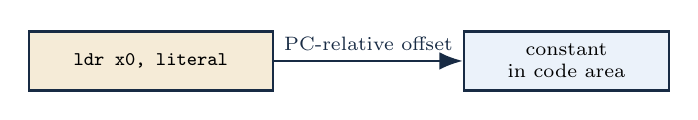
\begin{tikzpicture}[
  font=\scriptsize,
  box/.style={draw=navy, line width=0.8pt, minimum height=0.75cm, align=center}
]
\node[box, fill=gold!18, minimum width=3.1cm] (insn) {\code{ldr x0, literal}};
\node[box, fill=lightblue, minimum width=2.6cm, right=2.4cm of insn] (lit) {constant\\in code area};
\draw[-{Latex[length=3mm]}, navy, line width=1pt] (insn.east) -- node[above,font=\scriptsize]{PC-relative offset} (lit.west);
\end{tikzpicture}
\end{center}

\vspace{0.2cm}

\begin{itemize}\setlength{\itemsep}{5pt}
  \item The instruction encodes where to find the constant relative to the PC.
  \item The loaded value is data, even though it may be placed near the code.
  \item Assemblers may create literal pools automatically when a constant does not fit a simple immediate form.
\end{itemize}

\end{frame}

% ============================================================
% Slide 26
% ============================================================

\sectiondivider{Topic 7}{Branch Encodings}

% ============================================================
% Slide 27
% ============================================================

\begin{frame}{Conditional Branch Encoding}

\begin{block}{Example Forms}
\[
\code{b.eq label}
\qquad
\code{b.lt label}
\qquad
\code{b.ne label}
\]
\end{block}

\vspace{0.1cm}

\begin{center}
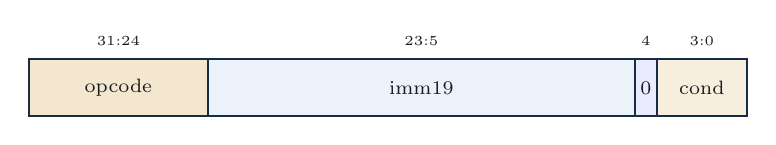
\begin{tikzpicture}[x=0.285cm,y=1cm]
  \bfld{0}{0}{8}{opcode}{gold!22}
  \bfld{8}{0}{19}{imm19}{lightblue}
  \bfld{27}{0}{1}{0}{blue!8}
  \bfld{28}{0}{4}{cond}{gold!15}
  \bitnote{4}{0.95}{31:24}
  \bitnote{17.5}{0.95}{23:5}
  \bitnote{27.5}{0.95}{4}
  \bitnote{30}{0.95}{3:0}
\end{tikzpicture}
\end{center}

\vspace{0.15cm}

\begin{itemize}\setlength{\itemsep}{6pt}
  \item The condition code is encoded in the low 4 bits.
  \item The signed immediate is 19 bits, scaled by 4 bytes.
  \item Conditional branches test the flags set by earlier compare or arithmetic instructions.
\end{itemize}

\end{frame}

% ============================================================
% Slide 28
% ============================================================

\begin{frame}{Conditional Branch Example: \texttt{b.eq}}

\begin{columns}[T,onlytextwidth]
\column{0.48\textwidth}
\begin{block}{Target Offset}
\[
\begin{aligned}
\text{current PC} &= \hex{100} \\
\text{target} &= \hex{110} \\
\text{imm19} &= 4
\end{aligned}
\]
\end{block}

\column{0.48\textwidth}
\begin{block}{Condition Field}
\[
\code{eq} = 0000
\]
The branch is taken when the Z flag is set.
\end{block}
\end{columns}

\vspace{0.2cm}

\begin{center}
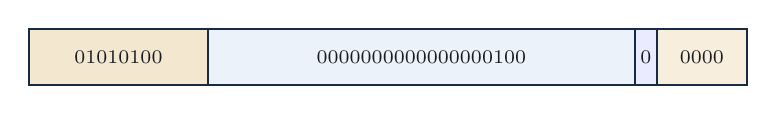
\begin{tikzpicture}[x=0.285cm,y=1cm]
  \bfld{0}{0}{8}{01010100}{gold!22}
  \bfld{8}{0}{19}{0000000000000000100}{lightblue}
  \bfld{27}{0}{1}{0}{blue!8}
  \bfld{28}{0}{4}{0000}{gold!15}
\end{tikzpicture}
\end{center}

\vspace{0.1cm}

\centering
\code{b.eq target} is encoded as \hex{54000080}.

\end{frame}

% ============================================================
% Slide 29
% ============================================================

\begin{frame}{Unconditional Branch Encoding}

\begin{block}{Instruction Forms}
\[
\code{b label}
\qquad\qquad
\code{bl function}
\]
\end{block}

\vspace{0.1cm}

\begin{center}
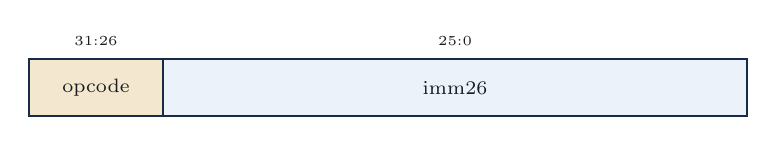
\begin{tikzpicture}[x=0.285cm,y=1cm]
  \bfld{0}{0}{6}{opcode}{gold!22}
  \bfld{6}{0}{26}{imm26}{lightblue}
  \bitnote{3}{0.95}{31:26}
  \bitnote{19}{0.95}{25:0}
\end{tikzpicture}
\end{center}

\vspace{0.15cm}

\begin{itemize}\setlength{\itemsep}{6pt}
  \item \code{b} and \code{bl} use a signed 26-bit immediate field.
  \item The offset is measured in 4-byte instructions, not raw bytes.
  \item \code{bl} also writes the return address into \code{x30}.
\end{itemize}

\vspace{0.1cm}

\begin{block}{Target Calculation}
\[
\text{target address} = \text{PC} + \operatorname{signextend}(\text{imm26}) \times 4
\]
\end{block}

\end{frame}

% ============================================================
% Slide 30
% ============================================================

\begin{frame}{Branch Example: Forward Target}

\begin{columns}[T,onlytextwidth]
\column{0.48\textwidth}
\begin{block}{Code Shape}
\small
\begin{tabular}{ll}
\code{0x100:} & \code{b target} \\
\code{0x104:} & \code{add x0, x0, \#1} \\
\code{0x108:} & \code{sub x1, x1, \#1} \\
\code{0x10c:} & \code{nop} \\
\code{0x110:} & \code{target:}
\end{tabular}
\end{block}

\column{0.48\textwidth}
\begin{block}{Offset}
\[
\begin{aligned}
\Delta &= \hex{110} - \hex{100} \\
       &= 16\text{ bytes} \\
\text{imm26} &= 16/4 = 4
\end{aligned}
\]
\end{block}
\end{columns}

\vspace{0.2cm}

\begin{center}
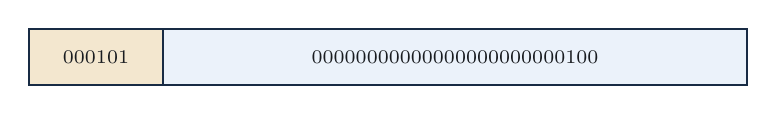
\begin{tikzpicture}[x=0.285cm,y=1cm]
  \bfld{0}{0}{6}{000101}{gold!22}
  \bfld{6}{0}{26}{00000000000000000000000100}{lightblue}
\end{tikzpicture}
\end{center}

\vspace{0.1cm}

\centering
\code{b target} is encoded as \hex{14000004}.

\end{frame}

% ============================================================
% Slide 31
% ============================================================

\sectiondivider{Topic 7}{Decoding and Reverse Engineering Machine Code}

% ============================================================
% Slide 32
% ============================================================

\begin{frame}{Decoding Checklist}

\begin{enumerate}\setlength{\itemsep}{8pt}
  \item Convert the hexadecimal word to 32 binary bits.
  \item Identify the broad encoding family from the opcode bits.
  \item Split the word into the fields for that family.
  \item Translate register fields into \code{x} or \code{w} register names.
  \item Interpret immediates carefully: sign extension, scaling, and shifts matter.
  \item Reconstruct the assembly instruction.
\end{enumerate}

\vspace{0.2cm}

\begin{block}{Important}
The same bit positions can mean different things in different instruction families.
Always identify the family before naming the fields.
\end{block}

\end{frame}

% ============================================================
% Slide 33
% ============================================================

\begin{frame}{Reverse Engineering Example}

\begin{block}{Given Machine Code}
\[
\hex{8B0700C5}
\]
\end{block}

\vspace{0.1cm}

\begin{center}
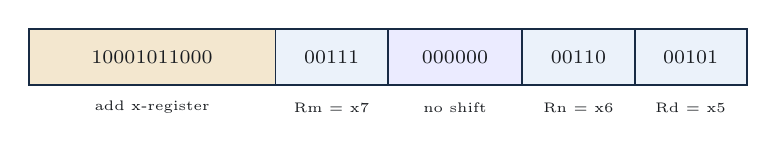
\begin{tikzpicture}[x=0.285cm,y=1cm]
  \bfld{0}{0}{11}{10001011000}{gold!22}
  \bfld{11}{0}{5}{00111}{lightblue}
  \bfld{16}{0}{6}{000000}{blue!8}
  \bfld{22}{0}{5}{00110}{lightblue}
  \bfld{27}{0}{5}{00101}{lightblue}
  \bitnote{5.5}{-0.28}{add x-register}
  \bitnote{13.5}{-0.28}{Rm = x7}
  \bitnote{19}{-0.28}{no shift}
  \bitnote{24.5}{-0.28}{Rn = x6}
  \bitnote{29.5}{-0.28}{Rd = x5}
\end{tikzpicture}
\end{center}

\vspace{0.35cm}

\begin{block}{Decoded Instruction}
\[
\hex{8B0700C5}
\quad\longrightarrow\quad
\code{add x5, x6, x7}
\]
\end{block}

\end{frame}

% ============================================================
% Slide 34
% ============================================================

\begin{frame}{Common Encoding Mistakes}

\begin{itemize}\setlength{\itemsep}{7pt}
  \item Treating a register number as decimal text instead of a binary field.
  \item Forgetting that AArch64 register fields are usually 5 bits.
  \item Encoding a byte offset directly when the immediate field is scaled.
  \item Applying the AArch32 \code{PC + 8} rule to AArch64 branch examples.
  \item Reading little-endian memory bytes as if they were the printed instruction word.
\end{itemize}

\vspace{0.2cm}

\begin{block}{Practical Habit}
Write the bit ranges first, then fill in the fields. Do not try to guess the final hexadecimal word too early.
\end{block}

\end{frame}

% ============================================================
% Slide 35
% ============================================================

\begin{frame}{Topic 7: Summary}

\begin{itemize}\setlength{\itemsep}{7pt}
  \item AArch64 instructions are fixed-width 32-bit words.
  \item The meaning of each bit field depends on the instruction family.
  \item Data-processing register instructions encode register operands and optional shift information.
  \item Data-processing immediate instructions use a different field layout.
  \item Load/store instructions commonly encode a base register, target/source register, and scaled offset.
  \item Branch instructions encode PC-relative offsets scaled by 4 bytes.
  \item AArch64 uses conditional branches and conditional operations rather than general per-instruction predication.
\end{itemize}

\end{frame}

% ============================================================
% Slide 36
% ============================================================

\begin{frame}{Self-Test Questions: Instruction Words}

\begin{enumerate}\setlength{\itemsep}{7pt}
  \item Why does AArch64 use 5-bit register fields?
  \item What is the difference between the printed hexadecimal instruction word and the byte order in memory?
  \item Why must the instruction family be identified before interpreting the fields?
  \item What fields are needed to encode \code{add x5, x6, x7}?
  \item Why does \code{add x5, x6, \#24} use a different format from \code{add x5, x6, x7}?
\end{enumerate}

\end{frame}

% ============================================================
% Slide 37
% ============================================================

\begin{frame}{Self-Test Questions: Memory and Branches}

\begin{enumerate}\setlength{\itemsep}{7pt}
  \item In \code{ldr x5, [x6, \#16]}, why is the encoded immediate 2 rather than 16?
  \item What is the role of \code{Rt} in a load? What is its role in a store?
  \item How is the target of an unconditional AArch64 branch computed?
  \item How does AArch64 conditional execution differ from AArch32 predication?
  \item Where is the condition code stored in a conditional branch instruction?
  \item Decode \hex{8B0700C5} back into the corresponding AArch64 assembly instruction.
\end{enumerate}

\end{frame}

% ============================================================
% Slide 38
% ============================================================

\begin{frame}{Looking Ahead}

\begin{block}{Next Topic}
Building a simple single-cycle RISC datapath.
\end{block}

\vspace{0.25cm}

\begin{itemize}\setlength{\itemsep}{7pt}
  \item Instruction fields become inputs to the datapath and control logic.
  \item Register fields select operands in the register file.
  \item Immediate fields must be extracted, extended, and routed.
  \item Branch offsets feed the next-PC calculation.
\end{itemize}

\end{frame}

\end{document}